\section{Design Strategy and Comparative Review}
To achieve the goal of developing an educational website that applies gamification principles to teach and promote recognition of open badges, this section is concerned with exploring design strategies, gamified elements, and supporting technologies.
While there is no exact example in the industry to follow for achieving this task, existing solutions of education and gamification applied in learning, digital badge systems will be reviewed, highlighting their core gamification features, similarities, and theories applied.

In addition to comparative analysis, this section examines layout logic, task design, and motivational models to inform the structure of the user experience. 
This includes a focus on layout and element design choices that prioritise clarity, responsiveness, and pedagogical intent, ensuring each interface component supports user engagement, progression, and learning outcomes.

Finally, software and technological tools are reviewed to support the implementation of verifiable badge issuance, ensuring that users who complete the website receive an open badge encoded with international metadata standards for recognition across the Web.

\subsection{Review of Existing Similar Solutions}
Existing similar solutions will be reviewed to identify key features, gamified elements, and theoretical strategies relevant to designing them. 
For the purposes of the project, the only concern is with educational, gamification and open badge integrations. 
The analysis will focus on platforms utilizing features such as badges, progress tracking, and leaderboards and the approach to their design to identify key elements and features to be implemented. 
To provide depth, theoretical frameworks like \acrshort{sdt}, \acrshort{mda} Framework, flow theory and alternative approaches will be explored in their application to these platforms. 
This review will adopt a comparative analysis approach, organizing findings into four core parameters: platform name, gamification approach and features, theoretical foundations or strategies applied, and relevance to project goals. 
Aspects like Target Audience, Accessibility, strengths and weaknesses as well as many other potential outlines will be ignored due to being considered out-of-scope for the project. 
Additionally, the selected products and services to-be-reviewed vary significantly in scope and application, so expanding the set of criteria to evaluate would lead to misrepresentation of certain criteria aspects.
By examining how these solutions address engagement and skill recognition, the review aims to conclude elements and strategies to inform the design of a gamified educational website about open badges. 
The following Table Parameters have been chosen:

\begin{itemize}
    \item \textbf{Platform Name and Type}:  Identity of the tool or platform and the type it represents.
    \item \textbf{Gamification and Features}:  Highlight applied game elements such as badges, leaderboards, progress tracking. Additional features, most notably open badge support and creation.
    \item \textbf{Theoretical Foundations or Strategies Applied}:  Examine the applied academic or practical design principles used to develop the features, to ensure evidence-based practices.
    \item \textbf{Relevance to Project Goals}: Explore relevance of application to the work, specifically in the field of recognition of achievement, recognition and integration of open badges. 
    This ensures that actionable features and strategies are identified.
\end{itemize}


\begin{longtable}[c]{|p{2.5cm}|p{4cm}|p{4cm}|p{4cm}|}
\captionsetup{justification=raggedright, singlelinecheck=false}
\caption{Comparative Analysis of Existing Platforms} \\
\hline
\textbf{Platform Name, Type} & \textbf{Gamification and Features} & \textbf{Theoretical Foundations or Strategies Applied} & \textbf{Relevance to Project} \\
\hline
\endfirsthead
\hline
\textbf{Platform Name, Type} & \textbf{Gamification and Features} & \textbf{Theoretical Foundations or Strategies Applied} & \textbf{Relevance to Project} \\
\hline
\endhead
\hline
\endfoot
\hline
\endlastfoot

\textbf{Mozilla Open Badges, Open Badge System} & Open badge creation, sharing, verification. Supports rich metadata, dictates international standards for issuing badges for educational accreditations. & Open recognition and learner autonomy principles, which tie into \acrshort{sdt}. The focus is on creating a standardized system for recognition, with an emphasis on verifiability and interoperability. & Provides the technical infrastructure needed to issue, verify, and share digital badges as well as the necessary metadata standards dictated. \\
\hline
\textbf{Badgr (Canvas Badges), Open Badge System} & Badge issuance, progress tracking, \acrshort{lms} integration, and social sharing options. & Use of badges, achievements and progress tracking aligned with \acrshort{sdt} and flow theory. & Supports easy digital badge creation, tracking of and rewarding learning achievements on manageable tracks, highly relevant for hassle-free digital badge creation. \\
\hline
\textbf{Open Badge Factory, Open Badge System} & Badge creation, issuing, and sharing, with reporting and data analysis features. & Encourages engagement through earning, tracking, and rewarding achievements. & Directly aligns with the goal of creating and recognizing open badges, offering a clear example of implementing badge metadata. \\
\hline
\textbf{Duolingo, Language Learning App} & Badges, streaks, Experience points, leaderboards, interactive lessons, various types of time-based, performance-based, task and progress tracking. & \acrshort{sdt} application - user autonomy, setup for achieving competence, relatedness through social systems, MDA Framework for driving engagement. & Engages users with gamified visual elements - badges, trackers, a map of Units. Supports skill recognition through milestones, suggests that having multiple ways of tracking progress is likely important for the user to keep track of their progress. \\
\hline
\textbf{Khan Academy, Educational Platform} & Progress tracking, mastery points, badges, personalized dashboards. & Mastery-based learning, flow theory for balanced challenges and skill levels. & Emphasizes clear progress indicators and personalized learning paths for user motivation. \\
\hline
\textbf{Coursera, Online Learning Platform} & Courses with progress tracking, certificates, community engagement. & Constructivist(enable users to construct their own understanding of the topic) learning, social learning, \acrshort{sdt} application for intrinsic motivation. & Combines certification and achievement systems, ideal for integrating open badges. \\
\hline
\textbf{Classcraft, Gamified Learning Platform} & Role-playing game mechanics (Experience, level-ups), collaboration, quests, and rewards. Includes avatars, team-based challenges, and behaviour tracking. & \acrshort{sdt} - focuses on competence through skill mastery, autonomy via customizable avatars and quests, relatedness through team-based interactions. & Encourages engagement and motivation through collaboration and role-playing elements, ideal for promoting both individual and group-based achievements. \\ \hline 
\textbf{Habitica, Task and Habit Tracker} & Gamified to-do list with tasks, streaks, and rewards. Users earn experience points and rewards for completing real-life tasks and goals. & \acrshort{sdt} application - intrinsic motivation through task completion and goal setting, competence through measurable progress, autonomy in managing tasks. & Provides a fun, gamified way to encourage habit formation and task completion, suitable for user achievement tracking in everyday activities. \\ \hline 
\textbf{Kahoot!, Game-Based Learning Platform} & Interactive quizzes, surveys, polls, leaderboards, and real-time gameplay in classrooms or teams. & Active learning principles, \acrshort{sdt} through engagement and social interaction in competitive settings. & Facilitates real-time, competitive learning, ideal for assessing knowledge and encouraging participation in educational settings. \\ \hline
\end{longtable}
{\raggedright \small{Source:} compiled by the author\par}

Platforms Mozilla Open Badges, and Open Badge Factory, which provide standardized badge creation and management systems are both viable options for issuing the work-related open badges for the purposes of the project. 
Badgr seems like a great addition that could go on to improve the experience with simple extra digital badges to explain the difference between digital and open badges. 
These systems align with the goal of the project for open recognition of the final badge and digital achievement recognition. 
Notably, research during development showed that Badgr is not a viable option due to technical limitations for badge issuing.

Gamified applications like Duolingo, Classcraft, and Habitica are focused on incorporating interactive elements such as streaks, quests, progress trackers and experience points to motivate users. 
By applying \acrshort{sdt}, these platforms effectively enhance intrinsic motivation through autonomy and competence (\cite{sdt}). 
Their emphasis on visual progress tracking and driving engagement highlights the importance of user-friendly interfaces for sustained participation. 
Duolingo’s gamified elements have been shown to increase user engagement and retention rates significantly according to Medium.com \footnote{https://medium.com/@theniteshknows/how-duolingo-reignited-user-growth-a-masterclass-in-gamification-strategy-2bc2d40e1876}.

Educational platforms Khan Academy and Coursera have developed personalized learning paths, mastery-based progress tracking, and social learning. 
These features are rooted in mastery learning, constructivist approaches, and active learning principles, which suggests the importance of personalized educational experiences that balance challenge and skill to maintain user engagement, per the flow theory (\cite{flow}, \cite{powerFeedback}). 
Unfortunately, personalising learning paths and creating extensive social learning opportunities would not be viable for the project due to limited scope and feasibility for both aspects. 
Kahoot! and Classcraft emphasise collaborative and competitive learning, team-based interactions and real-time participation to encourage both individual and group achievements. 
While team-based interactions are also considered out-of-scope for the project, there is the opportunity to implement the playfulness of presenting educational content like they are done in both of these platforms to improve the user experience.

These platforms illustrate a range of strategies that can inform decisions in both the design and technical implementation phases. 
Overall, the findings suggest that combining the structured credentialing of open badge systems with the engaging, user-centric design of gamified platforms can create an intuitive framework for motivated learning. 
These strategies and practical insights will serve as the foundation for designing an educational platform that integrates gamification and achievement recognition to drive both user engagement and educational outcomes.

\subsection{Gamification Frameworks and Applied Design Principles}
A growing number of educational platforms use gamification principles not only to attract attention but also to maintain engagement and reinforce learning outcomes. 
Progression systems and in-platform economies, as seen in platforms like "Cookie Clicker", demonstrate how users can be motivated to return through continuous visual and reward-based feedback over long periods. 
Although such systems originate in entertainment-focused products, their structural logic has informed many educational platforms by promoting retention through incremental achievements.

Research and industry commentary, such as a blog by \textcite{UXdesign}, emphasize the role of gamification in improving user experience and driving repeat interaction in digital learning environments. 
Browser-based educational tools like "Prodigy" successfully use rewards and incremental task-based challenges to engage younger audiences, demonstrating the power of good pacing in content releases.

Some early examples, such as Facebook-native games like "Farmville", were built primarily for keeping users terminally online as long as possible to maximise ad-revenue rather than have instructional value. 
These methods for sustaining engagement have influenced broader web development practices in terms of visual progression, feedback timing, and session structuring.

These patterns indicate that gamified educational platforms benefit most from clearly segmented user journeys with task-based progression, consistent feedback, and visible performance tracking. 
As supported by studies on digital engagement (\cite{userEngagement}, \cite{gamificationEngagement}), these features contribute to user motivation and platform familiarity. 

For this project, such implications informed the decision to implement a point-based task structure, sequential progression, and feedback mechanisms based on established gamification frameworks. 
The design aligns with the \acrshort{mda} framework by integrating game mechanics (task rules), dynamics (user interaction over time), and aesthetics (emotional feedback from scoring and badges). 
In parallel, \acrshort{sdt} (Self-Determination Theory) guided the structure toward autonomy and competence, while flow theory ensured tasks remained balanced in challenge and engagement (\cite{sdt}, \cite{flow}). 
These models collectively shaped the platform's reward logic and interaction flow. 

Beyond game design theories, the Fogg Behavior Model (\acrshort{fbm}) was also used to inform interface logic and user flow. 
FBM emphasizes the relationship between motivation, ability, and triggers (\cite{fogg}), suggesting that action occurs when users are sufficiently motivated, capable, and prompted at the right time. 
It also suggests that the challenge provided to the user has to progressively increase alongside the user's familiarity and knowledge of the challenge. 
A visual representation of the model is shown in Figure \ref{fig:foggChart}, illustrating the balance required for effective user engagement.
\begin{figure}[htbp]
 \centering
 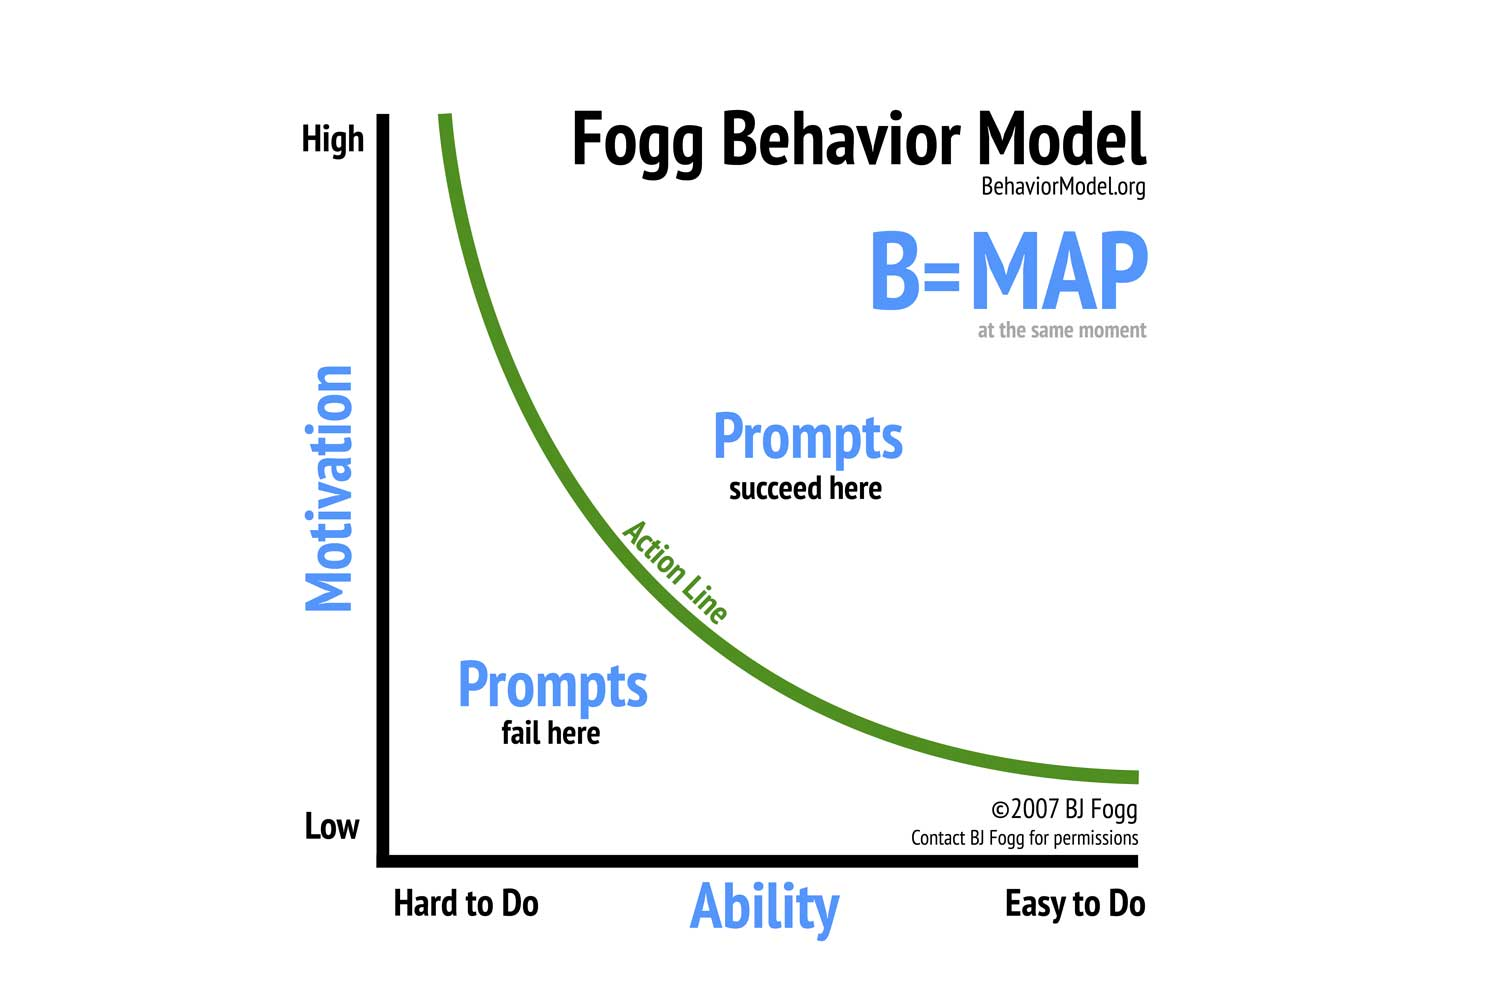
\includegraphics[width=14cm]{Media/Fogg-Behavior-Model.jpg}
 \caption{Fogg's Behavior Model}
 \label{fig:foggChart}
 {\raggedright \small{Source:} behaviormodel.org, 2009\par}
\end{figure}

\subsection{Layout and User Flow Decisions}
In the early design phase of the gamified educational website, low-fidelity wireframe designs were created to explore potential layout logic, user interaction flow and screen constraints, specifically for a mobile-first layout. 
These initial prototypes were primarily created in Figma, with mockups representing individual screen states across the core gamified tasks, such as the one shown in Figure \ref {fig:mockups}. 
Wireframes played a crucial role in identifying key user interface (UI) elements, narrative progression elements, and ensuring functional zones and compatibility for gamified interaction.

\begin{figure}[H]
  \centering
  \begin{subfigure}[]{0.3\textwidth}
    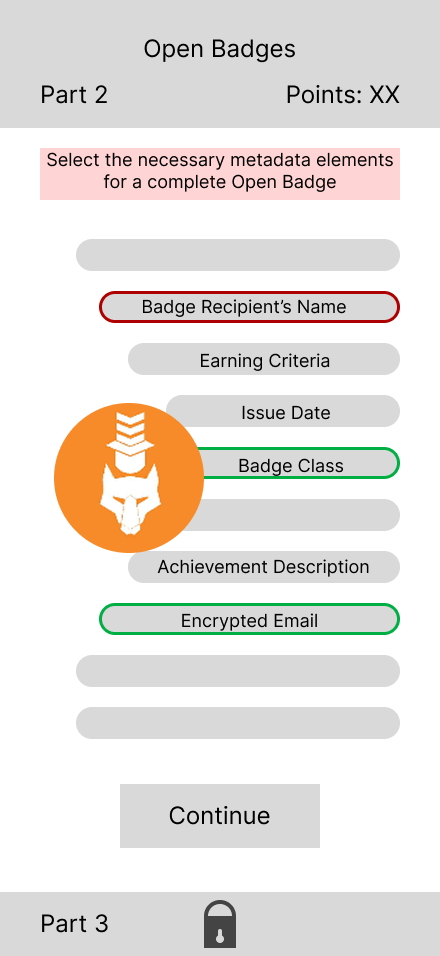
\includegraphics[width=\textwidth]{Media/design1.png}
    \caption{Task 1: Metadata selection}
  \end{subfigure}
  \hfill
  \begin{subfigure}[]{0.3\textwidth}
    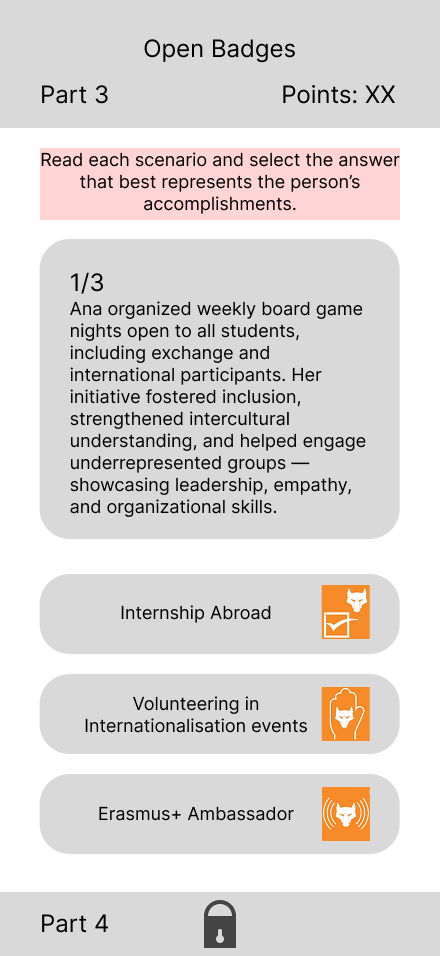
\includegraphics[width=\textwidth]{Media/design2.png}
    \caption{Task 2: Scenario choice}
  \end{subfigure}
  \hfill
  \begin{subfigure}[]{0.3\textwidth}
    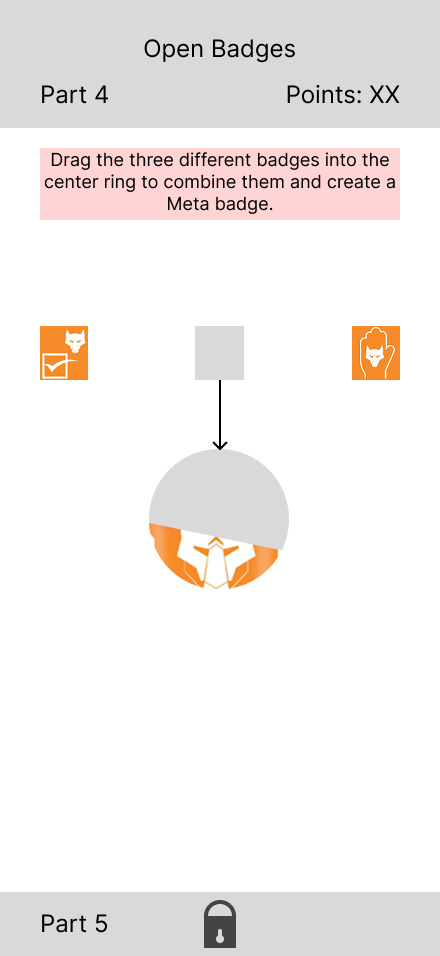
\includegraphics[width=\textwidth]{Media/design3.png}
    \caption{Task 3: Meta badge creation}
  \end{subfigure}
  \caption{Mobile UI mockups showing key gamified tasks}
  \label{fig:mockups}
  {\raggedright \small{Source:} created by the author\par}
\end{figure}

The overall layout of the gamified website was designed to support focused, step-by-step learning with minimal distraction. 
Some of the decisions were due to technical reasons; others, like a one-page structure, were product requirements specified by the supervisor.
Each design decision is made with the goal to emphasise clarity, responsiveness, and gamified interactivity, aligning both with pedagogical goals and user experience standards.

\subsubsection{Detailed Design Decisions}

\begin{itemize}
    \item \textbf{One-Page Scrollable Structure}: The website is planned to be a single scrollable page to maintain narrative continuity and reduce navigation complexity. 
    This promotes immersion by guiding users through a structured sequence without requiring manual or automatic page changes and allows for a strictly guided experience. 
    It also allows for lazy loading\footnote{A form of pre-loading where the website is instructed to load resources only when extra throughput is available and the core elements that the user is viewing are already loaded.} of visual elements such as the merge animation video that improves the stability and performance of the website. 
    Additionally, it is one of the initial requirements set for the project. 
    \item \textbf{Scroll Snapping Between Sections}: A series of anchor systems and respective elements were designed alongside a set of buttons to scroll between them. 
    In essence, each section holds an anchor <div> vertical element of the size of 1 pixel with respective offsets. 
    Each task has a button that either aligns the task to fill up the screen fully and consistently for the user or aligns the content for more comfortable reading. 
    It will work in each task individually, but there are additional buttons that help traverse sections at the start and end of the website. 
    This technique reinforces the concept of discrete “levels” or learning stages and prevents partial, out-of-context views of adjacent sections. 
    A post-development note is that scroll snapping was explored in-depth, and originally it was intended to lock the full website in scroll-snapping motion, but further investigation led to poor performance for either mobile or desktop users. 
    While the website is intended as mobile-first, creating a poor experience for the rest of the users is not viable or reasonable here and so a fraction of the intended solution has been implemented instead.
    \item \textbf{Task-Based Segmentation}: Content is divided into modular, self-contained tasks, each with its own interactive mechanics and feedback. 
    This segmentation mirrors gamification principles, providing a clear sense of progress and achievement at each step. 
    It functions as a level-based system that the user gets to progress through.
    \item \textbf{Mobile-First Responsive Layout}: The interface will be designed from the beginning to function on small screens, due to around 70\% of websites today being viewed on a mobile device according to Research.com \footnote{https://research.com/software/guides/mobile-vs-desktop-usage}. 
    Interactive elements have to be touch-optimised, which is discussed later in more detail. 
    Additionally, elements are vertically stacked and dynamically scaled, ensuring usability across a range of devices.
    \item \textbf{Colour-Guided Interactivity}:  The interface uses distinct colour signals (deep blue, yellow, green/red) to distinguish structural elements, guide attention, and provide immediate correctness feedback, supporting an intuitive, quick, comprehensible, and accessible user experience.
    \item \textbf{Integrated Feedback and Visual Cues}:  Feedback mechanisms such as visual popups, overlays, task completion percentages, score increases or decreases, animation effects and visual flair are embedded into the layout in ways to empower the user and respectively guide them through the experience. 
    These reinforce user actions and promote continued engagement.
    \item \textbf{Content Locking and Sequential Unlocking}:  Later sections of the website remain inaccessible until previous tasks are completed, reinforcing a mastery-based progression model. 
    This prevents skimming or skipping ahead and encourages focused engagement with each concept. 
\end{itemize}

\subsection{Element Design}
The design of individual interface elements throughout the website was primarily function-driven, where aesthetic decisions are made to support clarity, usability, and user feedback. 
Colours, shapes, and placements are selected not for ornamentation but to reinforce interaction goals, task structure, and user guidance. 
Typography is deliberately left minimal, relying on system defaults for simplicity and consistency across devices.

The visual identity of the website was structured to align with the university's branding while enhancing usability through consistent colour coding. 
Deep blue serves as the primary institutional theme colour, providing structural consistency across navigation, section headers, and tasks. 
Yellow is used as an accent to direct attention, applied to call-to-action, or \acrshort{cta} buttons and instructional highlights such as task descriptions, or form submission and website reset buttons. 
As an established interface design principle, green and red is used to indicate task correctness for immediate, intuitive feedback to learners. 
This structured use of colour reduces cognitive load and reinforces motivation by making task outcomes clear.

Elements are laid out in a vertically stacked structure, optimised for mobile interaction, with touch-friendly zones, consistent padding to ensure accessibility across devices. 
These spatial choices are supported by scroll-activated features, such as an animated Scalable Vector Graphics, or \acrshort{svg} zigzag path that is present within the introductory section and progressive unlocking of tasks, that visually signal user advancement. 
Conversely, a website reset is available after completion, which triggers a complete fadeout upon resetting user progress, to better convey the outcome. 
These mechanisms are designed not merely for aesthetics but to support learner motivation and focus, aligning with gamification principles that emphasise immediate, goal-oriented feedback as defined by \cite{redefinition}.

Buttons are styled using a visual hierarchy based on their function. 
Primary actions, such as progressing through tasks or claiming a badge, are styled as yellow, circular buttons, ensuring high contrast and immediate visibility. 
These stand in contrast to outlined or subdued secondary buttons in deep blue, which are used for auxiliary navigation within tasks or task buttons themselves. 
This hierarchy reduces the likelihood of user confusion and subtly guides attention toward key learning actions.

Interactive zones within tasks are also shaped by their function. 
For example, drag-and-drop areas are outlined with dashed or shaded containers to suggest manipulability, while static information zones are clean and visually neutral. 
Pop-up feedback components, such as correction prompts or success confirmations, follow a consistent form with a lightly elevated overlay with clear textual content and contextual visual cues. 
These design elements help distinguish between active, passive, and reactive interface components, enhancing overall clarity.

Finally, the visual hierarchy of the system is intentionally kept thin. 
Task screens aim to present no more than two or three levels of importance at any time (e.g., a task prompt and an interaction area, optional tooltip). 
This supports cognitive load minimisation and aligns with pedagogical priorities, critical in gamified learning contexts where distraction can reduce instructional effectiveness (\cite{reduceDistraction}).

\subsection{Pedagogical Strategies and Task Design}
The website was designed with the goal to maintain user motivation, support meaningful engagement, and deliver instruction through concise, interactive segments. 
Gamification principles outlined previously were integrated to reinforce motivation and progression, while educational effectiveness was achieved through a structured set of tasks, each emphasising a distinct learning objective.

To encourage continuous engagement, the platform includes gamified components such as progress tracking, a point-based scoring system, and a feedback loop. 
Progress bars appear within tasks where necessary, providing a visual sense of advancement. 
The scoring system rewards correct answers and penalises incorrect ones, with scores later submitted as part of the badge qualification process in the form of criteria, incentivising focused attention on the provided learning materials. 
Users also receive feedback in the form of overlay notifications if they attempt to access locked content before completing prior steps, reinforcing the structured, on-rails experience.

The learning journey is organised into five distinct task types, each tailored to test and reinforce different aspects of the open badge concept:
\begin{itemize}
    \item \textbf{Card Classification:} Categorizes competencies into hard and soft skills, with the strict association between open badges and soft skill competencies.
    \item \textbf{Element Selection:} Involves choosing correct badge metadata from visual options.
    \item \textbf{Scenario Selection:} Challenges users to apply badge knowledge to realistic decision-making contexts.
    \item \textbf{Item Combination:} Visually demonstrates the concept of combining badges into a larger "Meta" badge of a different badge class.
    \item \textbf{Card Association:} Requires categorising cards with the relevant stakeholder benefiting from the outlined concept.
\end{itemize}

To reduce onboarding friction, minimal guidance is provided via tooltips and progressive task visibility. 
Scenario-based interactions and interactive quizzes are used to convey concepts dynamically, mirroring real-world applications of open badges and encouraging decision-based learning. 

Supporting features such as SVG animations, visual cues are included to aid navigation and provide a smooth, intuitive experience. 
The platform is localised in both Lithuanian and English to improve accessibility. 
Additionally, earned badges are distributed via email and must be actively claimed by the user, reinforcing the reward structure and providing a tangible outcome to the learning process.

As a final reinforcement mechanism, users receive an open badge upon completing the full learning sequence. 
These badges are issued in compliance with international metadata standards, ensuring they carry both symbolic and verifiable value. 
The ability to export and share these credentials adds an extrinsic motivational layer, encouraging learners to complete the content not only for the experience itself but also for a transferable proof of achievement. 
This aligns with trends in microcredentialing and digital recognition in education.

\subsection{Software Solution Review}

When planning the required technologies that could support both the pedagogical and gamified goals of the project, rather than committing to fixed tools from the outset, the software solution review focused on tool categories and their ability to meet responsiveness, interactivity, and credentialing requirements.

Several web development technologies were considered for frontend design, including component-based frameworks such as React.js, due to their flexibility in building modular and dynamic user interfaces. 
Backend considerations focused on scalability and ease of API integration, especially for badge issuance and event tracking, leading to the selection of lightweight Node.js-based frameworks.

API integrations supporting the Open Badge standard were explored, with services like Open Badge Factory offering reliable support for metadata-rich badge issuance and delivery workflows.
Vilnius Tech's open badge provider badgecraft.eu and Badgr were also considered but were not viable during development due to certain technical constraints. 
Technical constraints include but were not limited to deprecated API access or missing API functionality.
For future implementation into the university's ecosystem, some adjustments are planned and would have to be made to fully function.

Browser-game engine Phaser 3 was considered for game creation, to have the users get involved even further, through quick and simple game sequences. 
This could range from online team-play to guiding users through learning new concepts about open badges.

Other auxiliary tools such as Git for version control, Jest for testing, and Lighthouse for accessibility review were also evaluated to ensure development best practices were met.

The final technology stack is presented in Section 3, including specific roles and deployment considerations.

\subsection{Design Strategy Summary}
This section outlined the comparative foundation and design rationale behind the development of the gamified educational website focused on open badge recognition. 
Existing platforms were analysed for their gamification features and educational strategies, providing theoretical grounding through models such as \acrshort{sdt}, \acrshort{mda}, flow theory, and the Fogg Behavior Model. 
These insights informed both layout and interface design choices, which emphasize mobile-first usability, interactivity, and feedback-driven progression. 
Each task was crafted to align pedagogical intent with motivational mechanics, culminating in the issuance of a verifiable open badge. Finally, appropriate technologies and tools were considered to support modular development, badge integration, and responsive delivery, setting the groundwork for the programming phase discussed in the following section.